\section{Simulation Analysis}
\label{sec:simulation}

\subsection{Operating Point Analysis}

Following our theoretical analysis, the circuit was simulated in the Ngspice software. 
In step (1), we were asked to simulate the operating point for t<0, in order to find the voltages in all nodes and the currents in all branches. The results are shown in Table~\ref{tab:alinea1}.

\begin{table}[h]
  \centering
  \begin{tabular}{|l|r|}
    \hline    
    {\bf Name} & {\bf Value [A or V]} \\ \hline
    \input{op1_TAB}
  \end{tabular}
  \caption{Operating point for t<0. Simulated Values for voltage (V) and current (A) using Ngspice.}
  \label{tab:alinea1}
\end{table}

Then, in step (2), we simulated the operating point considering that the voltage of the source in the instant t=0 was null and replacing the capacitor with a voltage source that was equal to V6-V8, being this values the voltages in the capacitor's nodes that were obtained in (1). This step was needed because... The results are shown in Table~\ref{tab:alinea2}.

\begin{table}[h]
  \centering
  \begin{tabular}{|l|r|}
    \hline    
    {\bf Name} & {\bf Value [A or V]} \\ \hline
    \input{op2_TAB}
  \end{tabular}
  \caption{Operating point for Vs=0 (instant t=0). Simulated Values for voltage (V) and current (A) using Ngspice.}
  \label{tab:alinea2}
\end{table}

In step (3), we simulated the natural response of the circuit. In Figure~\ref{fig:plotS(3)} we can find the plot of v6 in the interval [0, 20]ms.

\begin{figure}[h] \centering
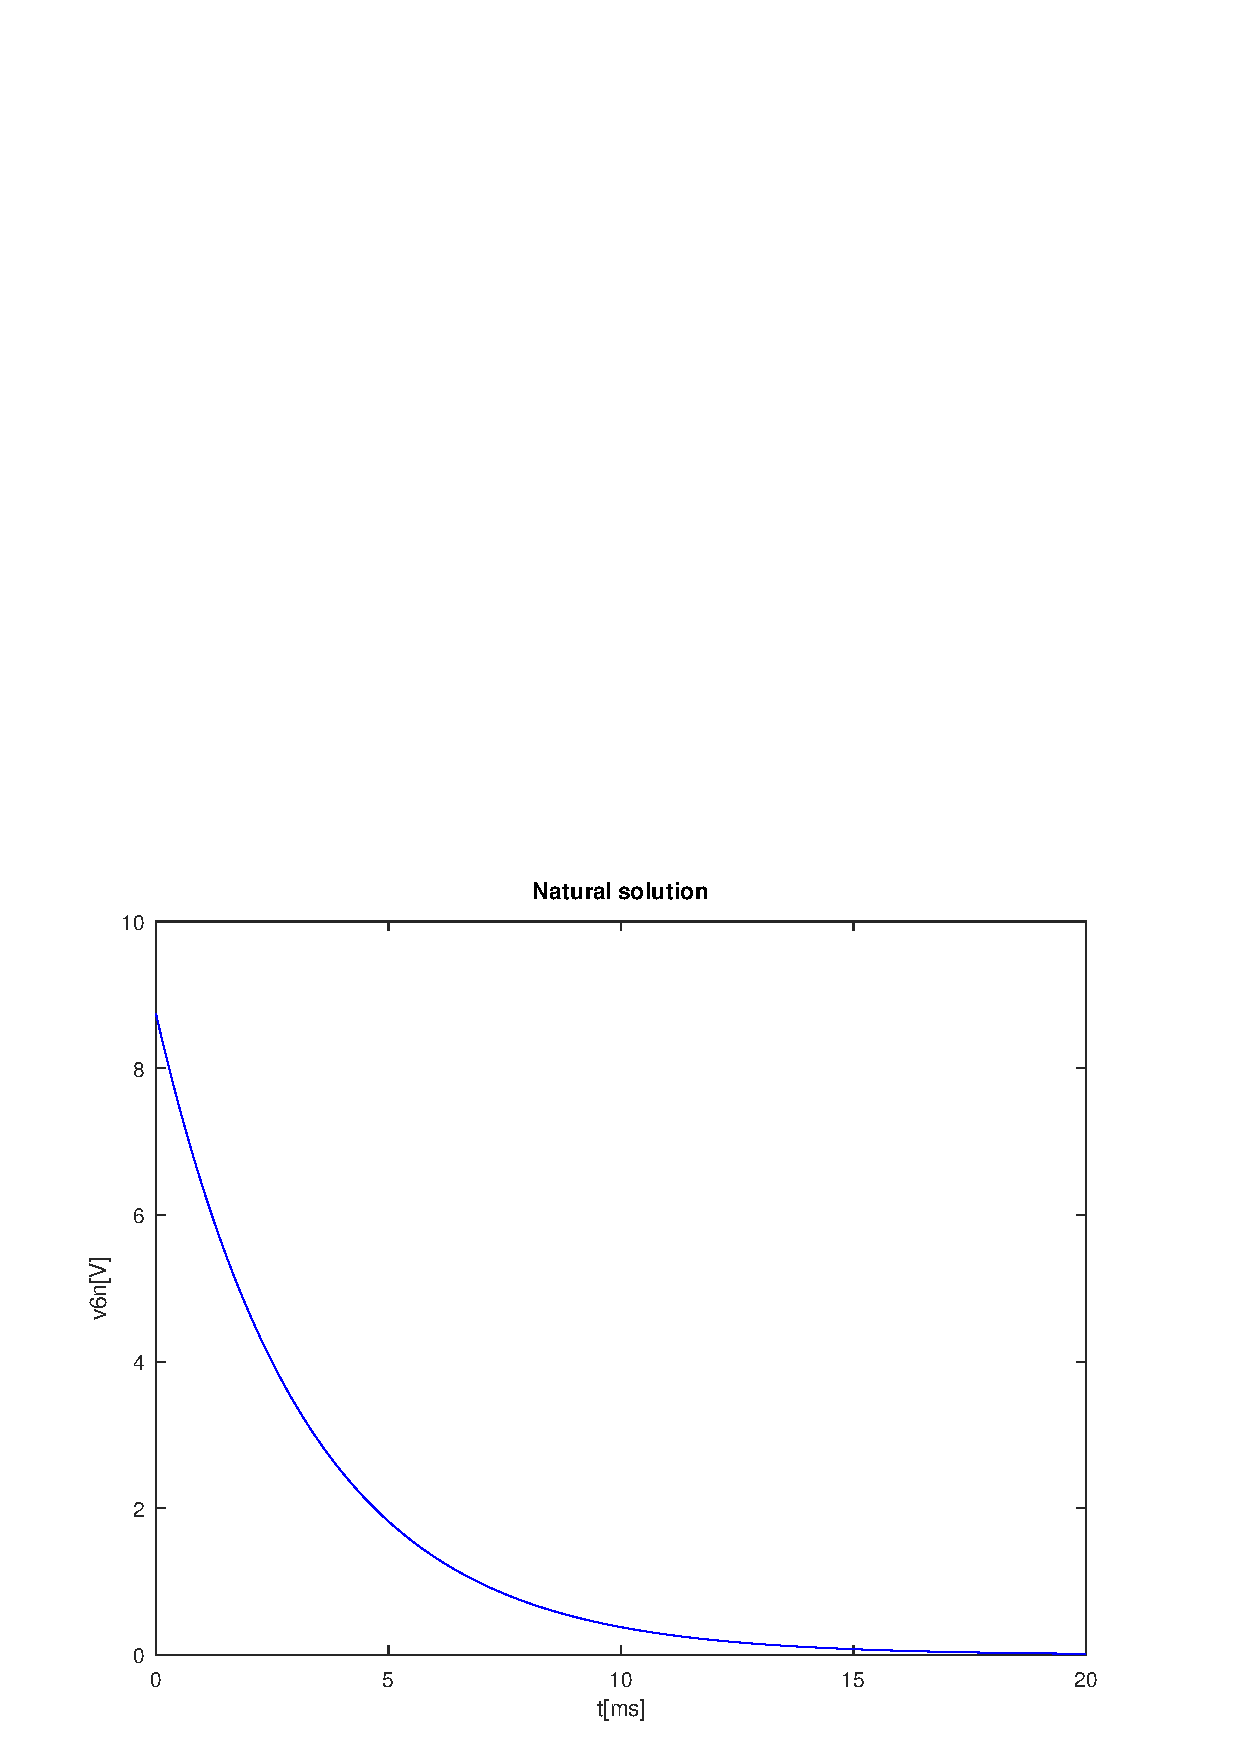
\includegraphics[width=0.8\linewidth]{naturalsolution.pdf}
\caption{Plot of v6(t) in the interval [0, 20]ms.}
\label{fig:plotS(3)}
\end{figure}

Later, in step (4), we were asked to simulate the natural and forced response on node 6 by repeating step (3) with vs(t) as given in Equation~\ref{eq:vs} and f=1kHz. In Figure~\ref{fig:plotS(4)} we can see the plot of both the stimulus and the response.

\begin{equation}
  V_{s}(t) = sin(2 \pi f t),
  \label{eq:vs}
\end{equation}

\begin{figure}[h] \centering
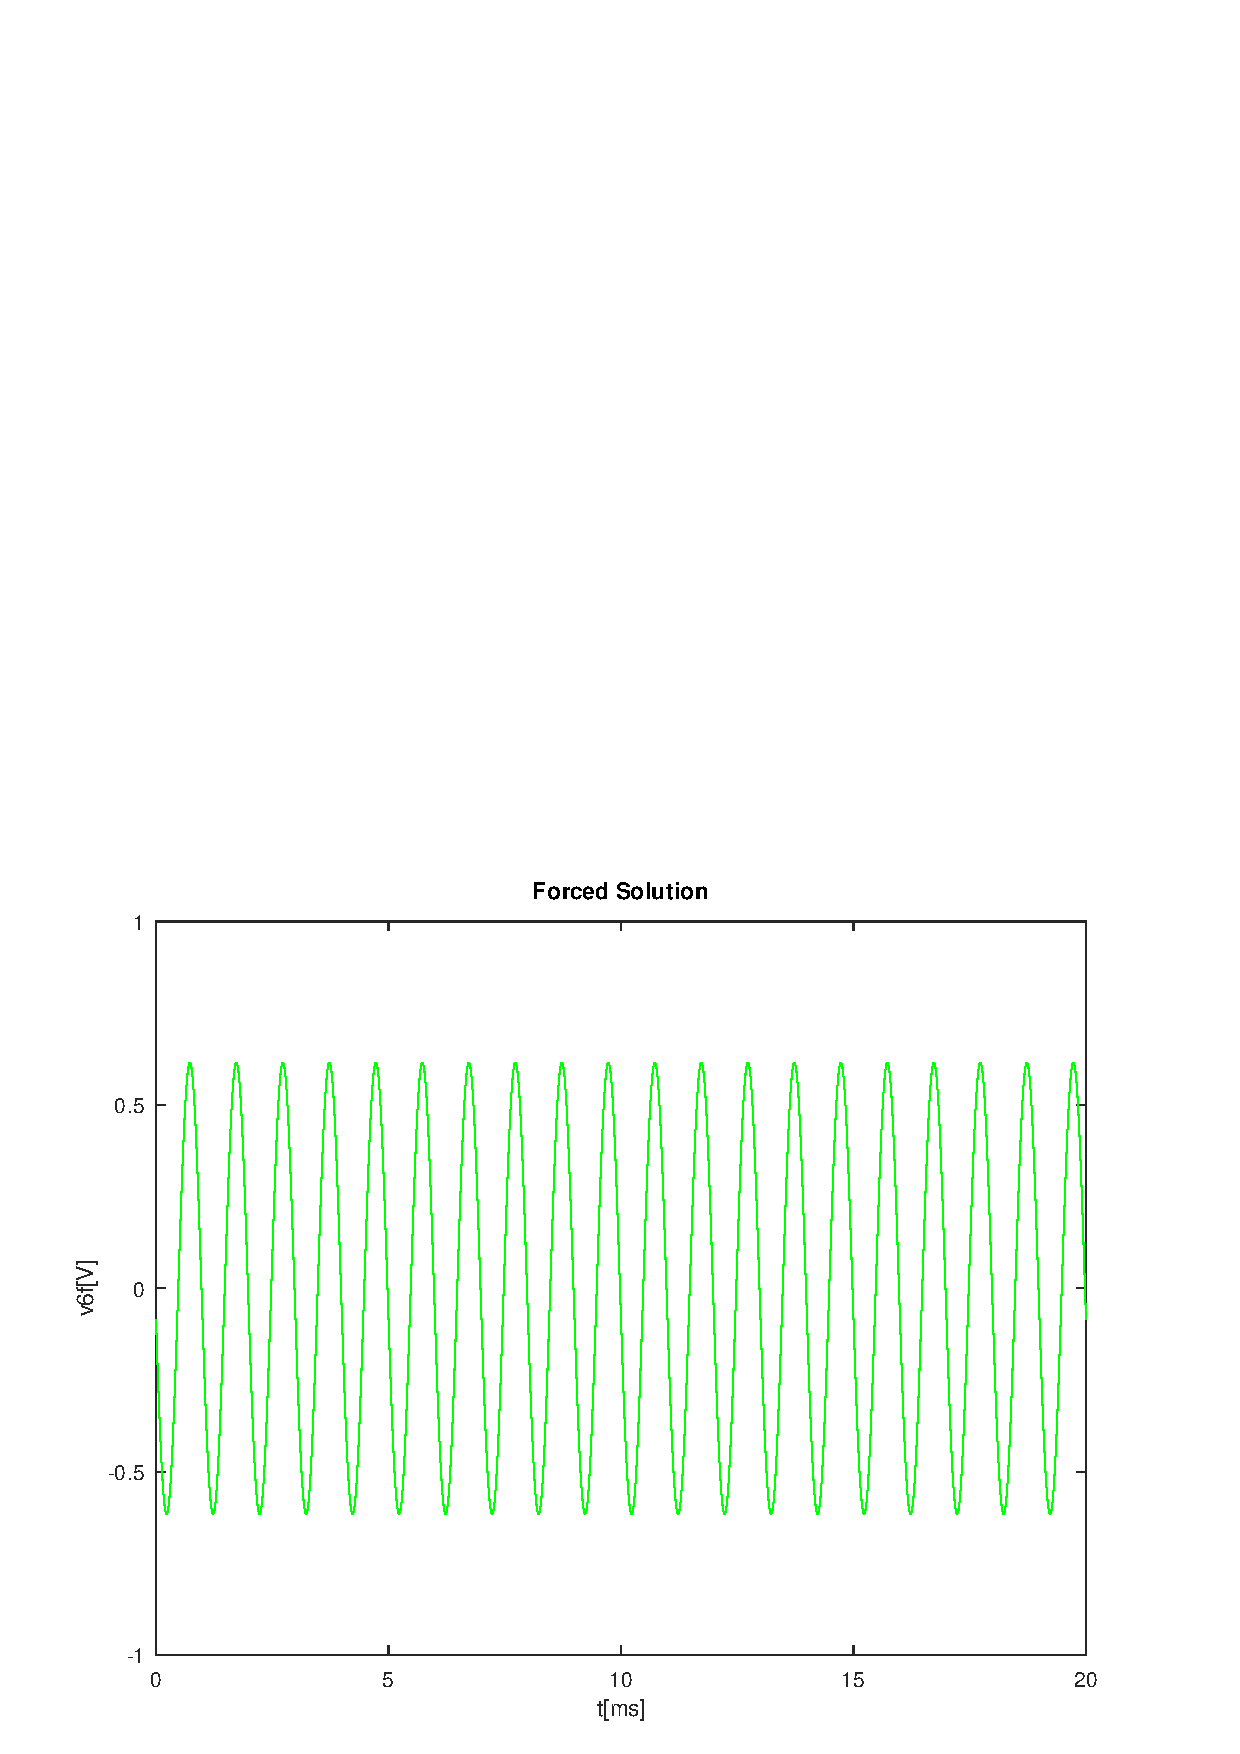
\includegraphics[width=0.8\linewidth]{forcedsolution.pdf}
\caption{Plot of v6(t) in the interval [0, 20]ms.}
\label{fig:plotS(4)}
\end{figure}

At last, in step (5), the frequency response in node 6 was simulated  for the frequency range 0.1 Hz to 1 MHz. In Figure~\ref{fig:plotS(51)} and Figure~\ref{plotS(52)} we plotted the amplitude frequency response and the phase response, respectively. It is important to notice that the frequency logscale as its magnitude in dB units and the phase is presented in degrees.

\begin{figure}[h] \centering
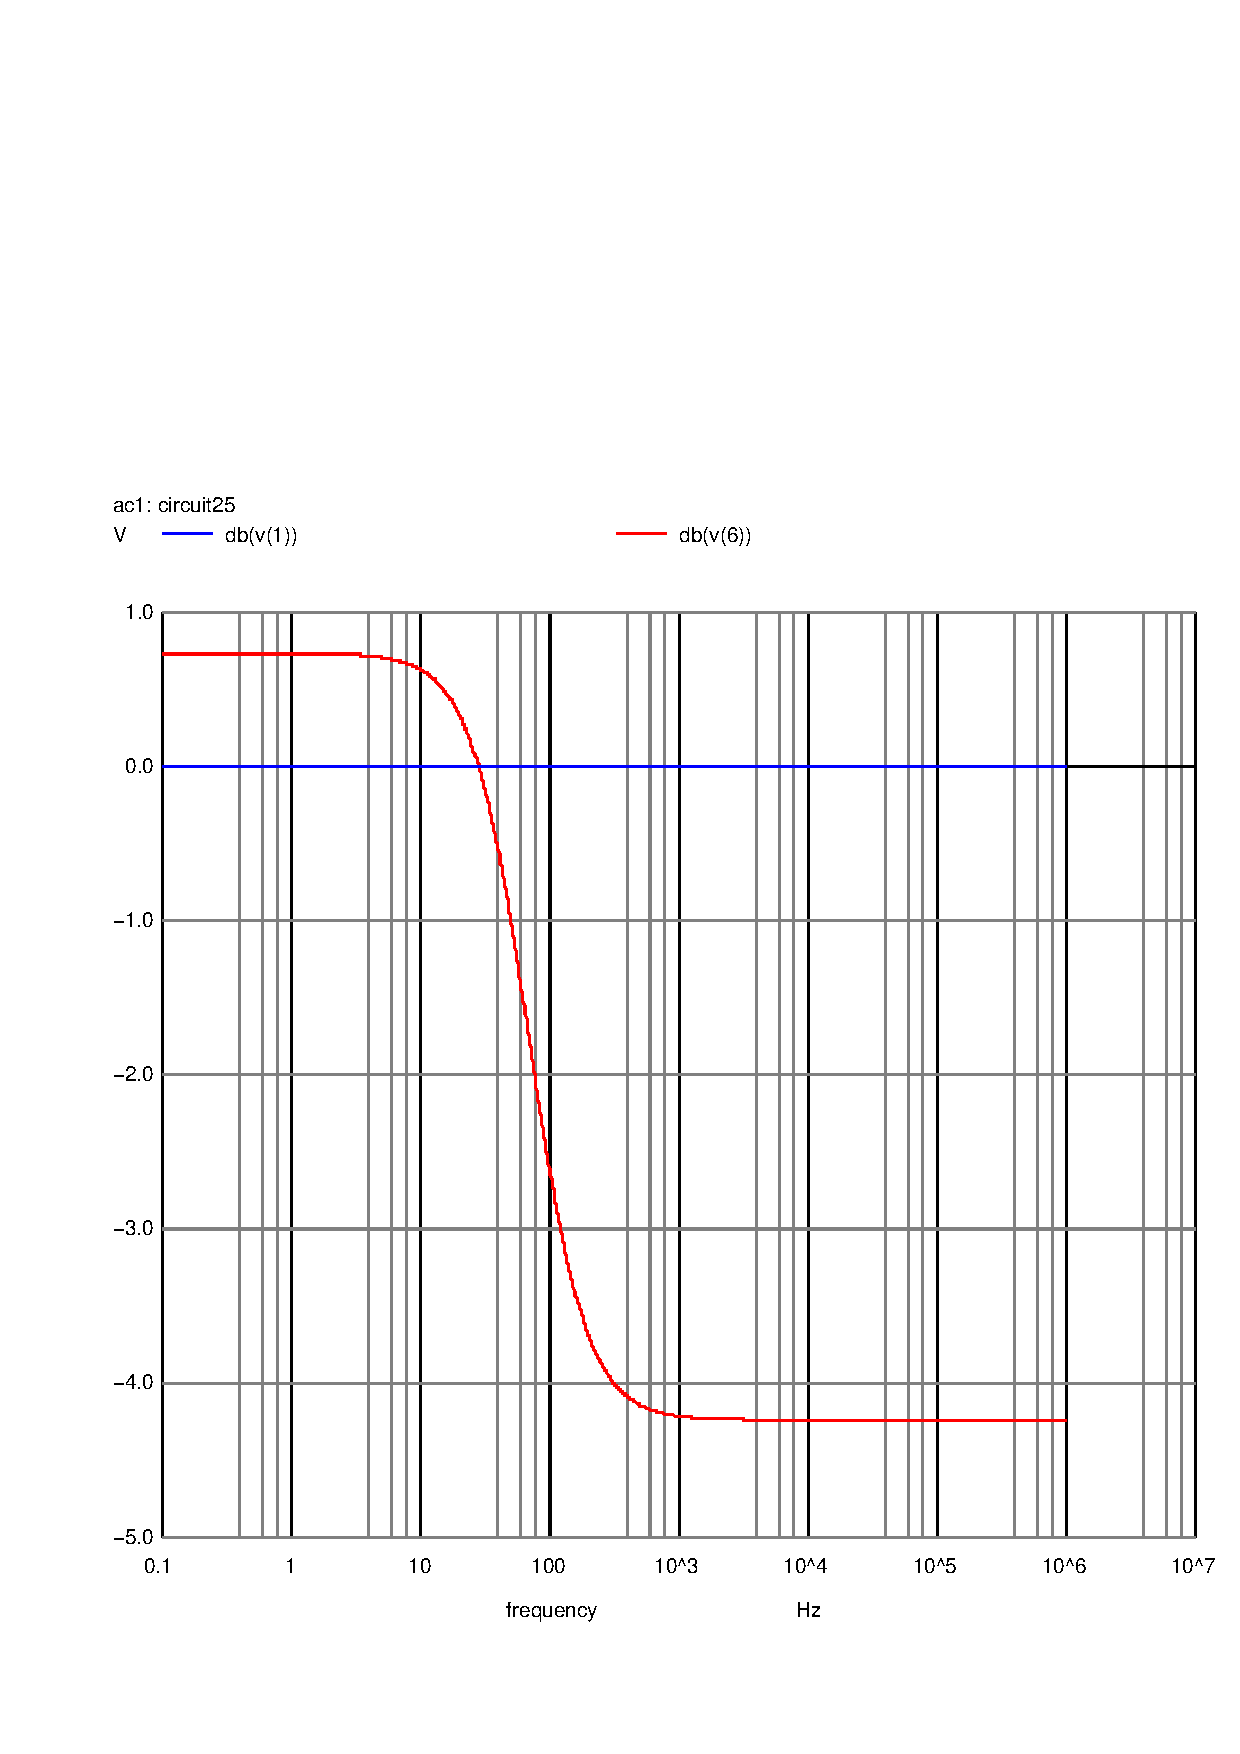
\includegraphics[width=0.8\linewidth]{ampresponse.pdf}
\caption{Plot of amplitude frequency response (for vs(f) and v6(f)) in the interval [0.1, 1M]Hz.}
\label{fig:plotS(51)}
\end{figure}

\begin{figure}[h] \centering
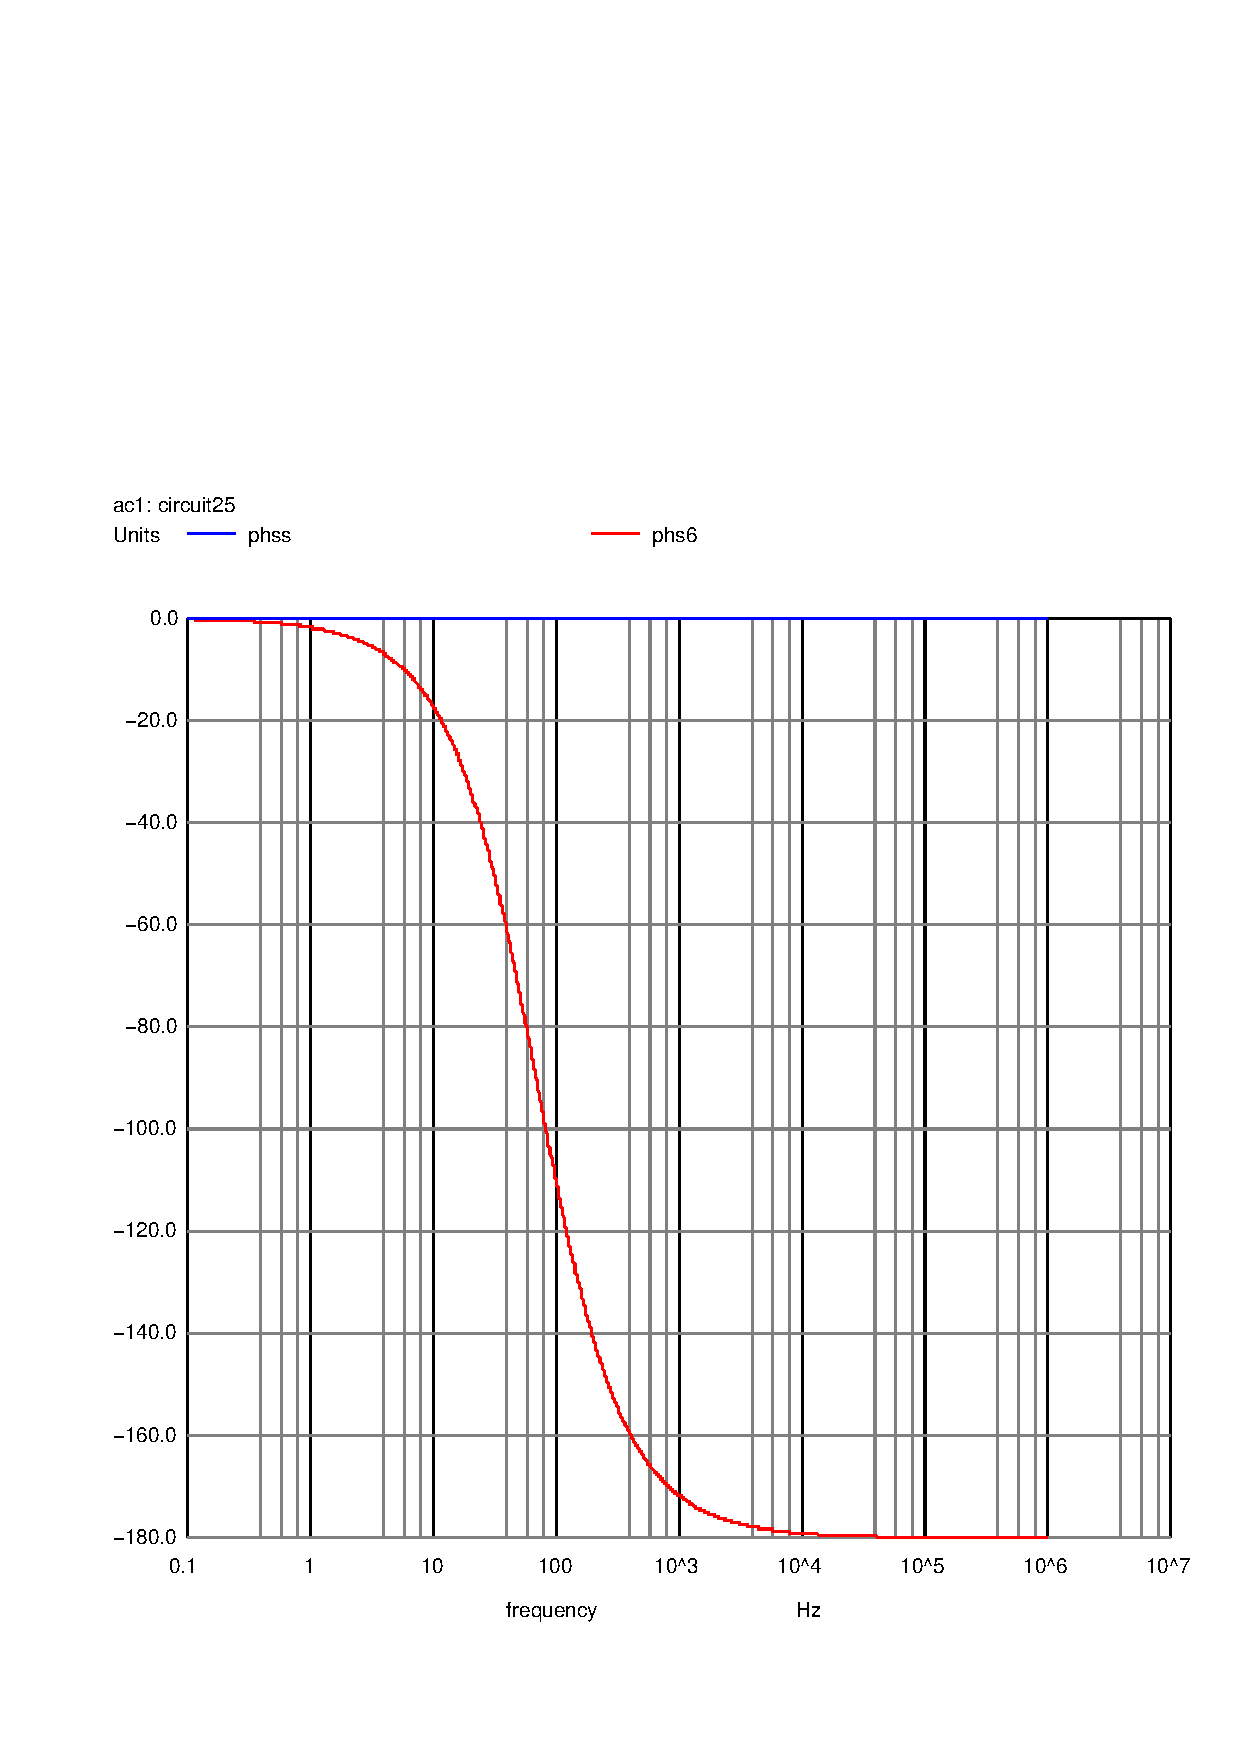
\includegraphics[width=0.8\linewidth]{phaseresponse.pdf}
\caption{Plot of phase response (for vs(f) and v6(f)) in the interval [0.1, 1M]Hz.}
\label{fig:plotS(52)}
\end{figure}

Just like was predicted in our theoretical analysis, by simulating we came to the conclusion that v6 and vs differ because of the reasons that were mentioned in the previous chapter.


